\section{Materials and Methods}
\label{sec:matmet}

In this section we present the materials used in the research - the British spatial
signatures used as to generate labels for individual chips and Sentinel 2 satellite
imagery - and methods designed to unpack the role of geography in image-based deep
learning.

\subsection{Materials}

The whole research uses only two data inputs, one representing the "ground truth" we are
aiming to predict using neural networks and the other representing the satellite
imagery. While the latter does not need a lot of introduction, the British spatial
signatures used as the labels need to be explained further.

\subsubsection{British Spatial Signatures}
% 500 words

Spatial signatures are a way of classification of space covering entirety of a case
study area. They are defined as \textit{"a characterisation of space based on form and
function designed to understand urban environments"} \citep{dab_mf_2021a} and the
definition already points at the clear distinction between signatures and traditional
Land Use / Land Cover (LULC) classifications. Taking the example of CORINE (REF) as a
representative of LULC, it has 44 distinct classes, out of which 2 cover urban form and
other 6 can be loosely related to urban areas\footnote{Continuous urban fabric,
Discontinuous urban fabric; Construction sites, Green urban areas, Sport and leisure
facilities, Industrial or commercial units, Road and rail networks and associated land,
Port areas}. A similar situation is with recently released global LULC datasets.
European Space Agency's WorldCover project distinguishes 11 classes of which one is
urban (Built-up) REF. Esri's Land cover has 9 classes where one is \textit{Built Area}
and the rest covers unbuilt areas REF. This ratio of built vs unbuilt classes is typical
but not very suited for research applications focusing on urban environments. Spatial
signatures tend to flip this ratio as they are primarily classifying urban space.

There are two key main concepts embedded in spatial signatures delivering urban-focused
classification. The first one is the spatial unit called the enclosed tessellation cell
(ETC). To derive ETCs, we first generate \textit{enclosures}, a space fully enclosed by
a set of barriers (roads, railways, rivers, coastline). ETCs are then a result of
Voronoi tessellation based on building footprint polygons. The resulting spatial unit
has adaptive granularity reflecting the scale of each individual urban pattern. The
second is the selection of characters describing each ETC. We measure form and function,
both primarily urban phenomena and mostly omit environmental aspects focusing on land
cover patterns.

% We may want to add a figure explaining ETCs here.

British spatial signatures are one application of the concept of spatial signatures in
the context of Great Britain REF SDATA. It divides the space into 16 data-driven classes
(figure \ref{fig:signatures}) listed in the table \ref{tab:sig_types}. Out of these 16
classes, 9 are entirely urban, 4 are peripheral and only 3 are classifying countryside,
completely flipping the ratio of built vs unbuilt classes known from LULC. However, out
of these 16 classes, some are very scarce and it would not be feasible to attempt to
predict them. Therefore, we merge 5 classes falling under the "urbanity" group into a
single one and use resulting 12 classes throughout this paper.


\begin{tabular}{lrrrr}
    \caption{\label{tab:sig_types}Classes of British spatial signatures and their
    coverage in terms of area and a number of ETCs.}\\
    \toprule
    {} &        total area (sq.km) &  total ETC count &  percentage of area &
    percentage of ETCs \\
    signature\_type                       &             &         &            &
    \\
    \midrule
    Countryside agriculture              & 93,856.1 & 3,022,385 &         41 &
    21 \\
    Accessible suburbia                  &  2,244.5 & 1,962,830 &          1 &
    14 \\
    Dense residential neighbourhoods     &    957.2 &   502,835 &          0 &
    3 \\
    Connected residential neighbourhoods &    565.4 &   374,090 &          0 &
    3 \\
    Dense urban neighbourhoods           &    570.6 &   238,639 &          0 &
    2 \\
    Open sprawl                          &  5,081.5 & 2,561,211 &          2 &
    18 \\
    Wild countryside                     & 91,306.3 &   595,902 &         40 &
    4 \\
    Warehouse/Park land                  &  2,462.4 &   707,211 &          1 &
    5 \\
    Gridded residential quarters         &    261.2 &   209,959 &          0 &
    1 \\
    Urban buffer                         & 31,588.8 & 3,686,554 &         14 &
    25 \\
    Disconnected suburbia                &    708.9 &   564,318 &          0 &
    4 \\
    Local urbanity                       &    231.1 &    86,380 &          0 &
    1 \\
    Concentrated urbanity                &      7.8 &     1,390 &          0 &
    0 \\
    Regional urbanity                    &     76.4 &    21,760 &          0 &
    0 \\
    Metropolitan urbanity                &     16.5 &     3,739 &          0 &
    0 \\
    Hyper concentrated urbanity          &      2.2 &       264 &          0 &
    0 \\
    \bottomrule
\end{tabular}



\begin{figure}
    \centering
    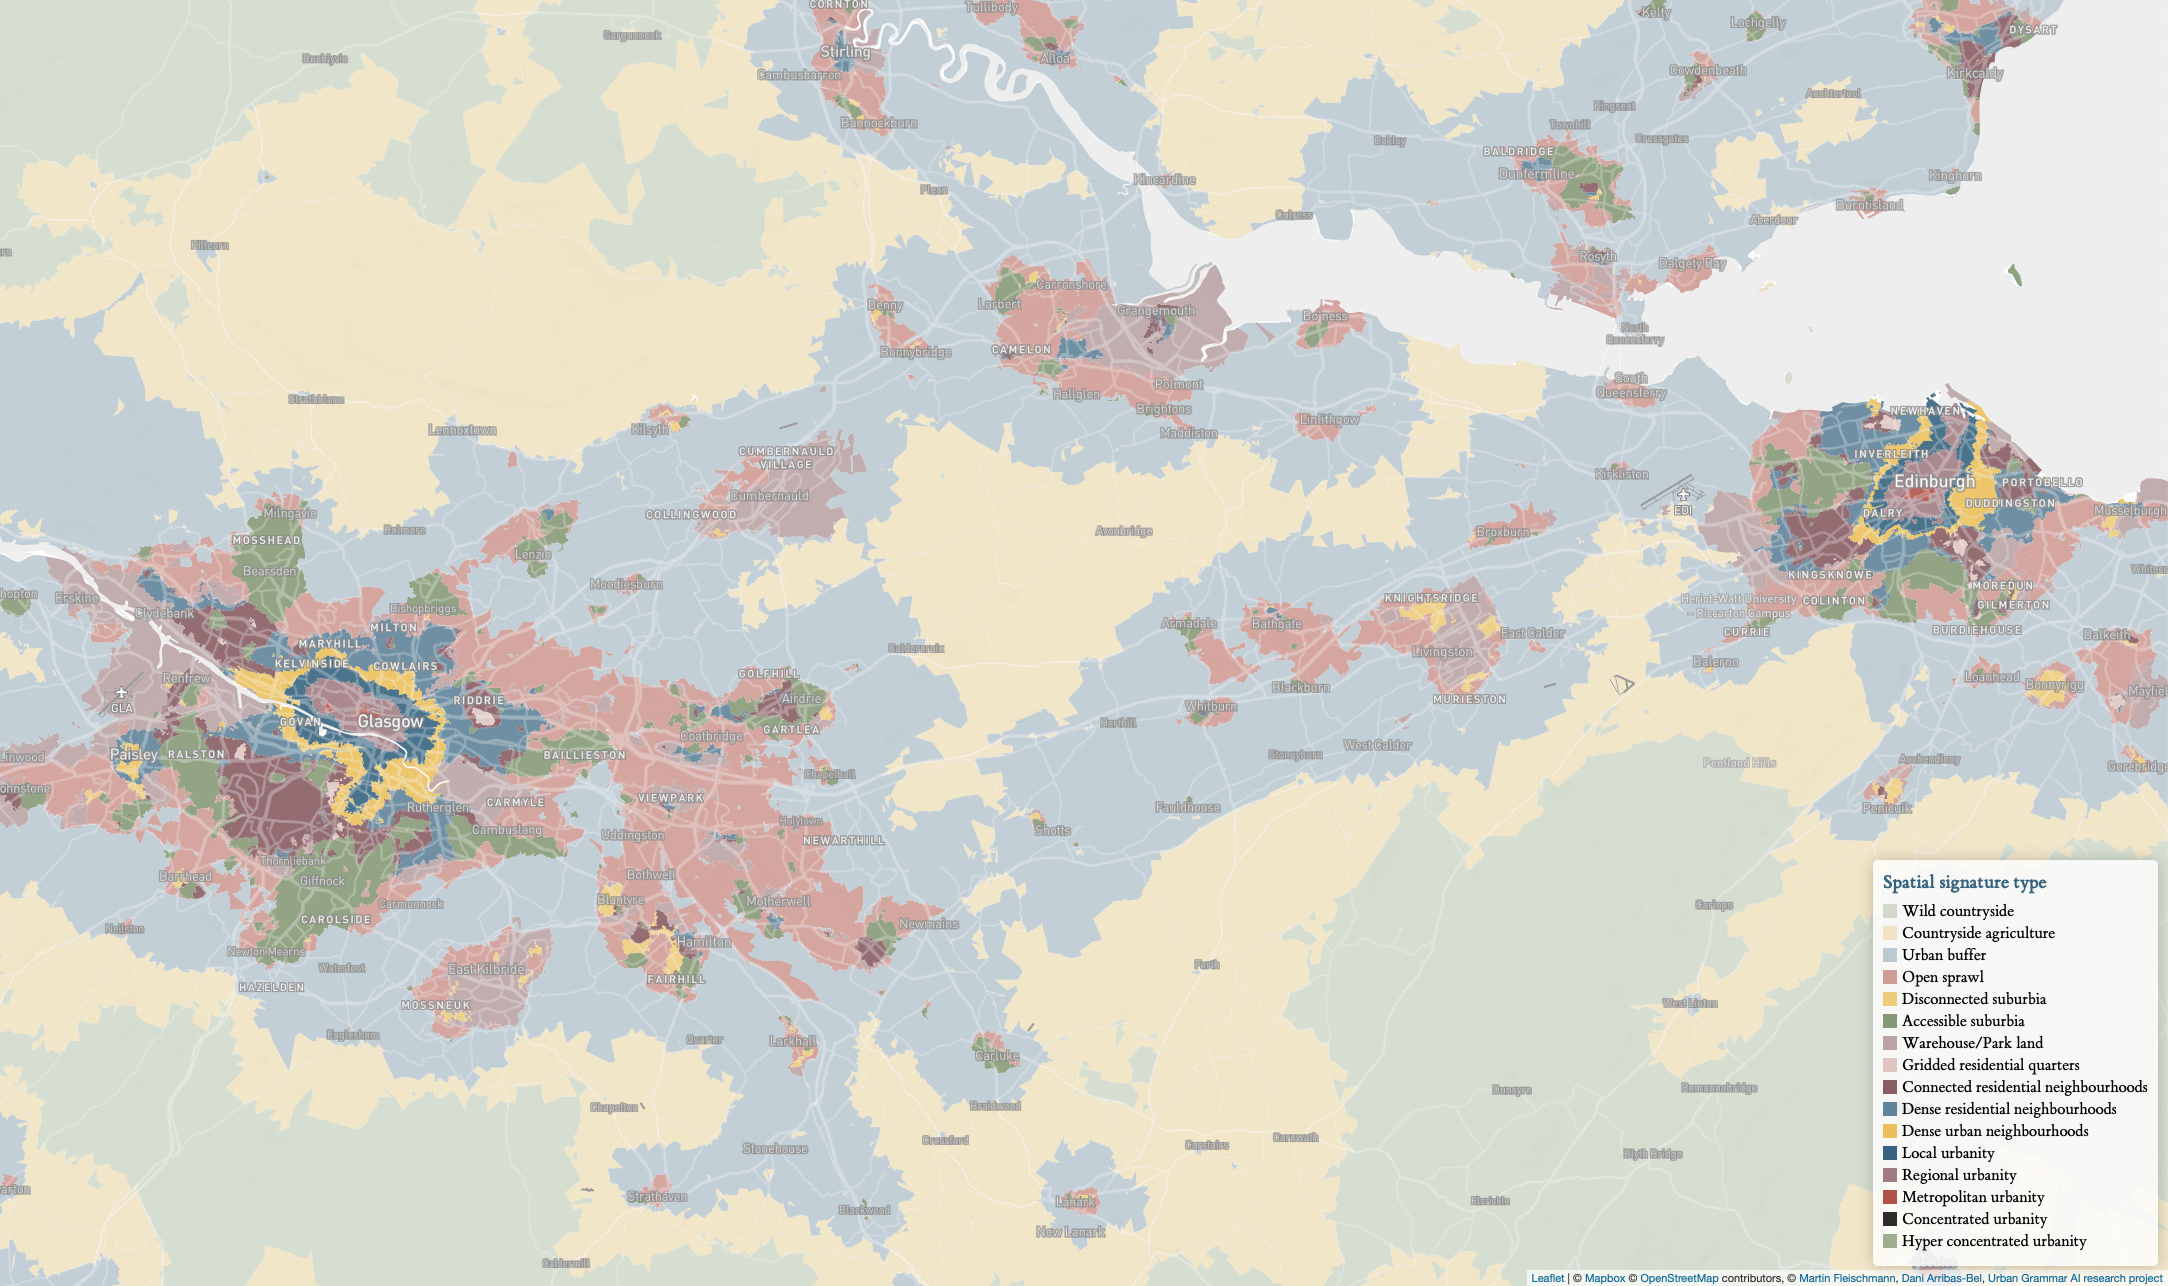
\includegraphics[width=.8\linewidth]{fig/signatures_scotland.png}
    \caption{Spatial signatures in the area of the Scottish Central Belt stretching from Glasgow to Edinburgh.}
    \label{fig:signatures}
\end{figure}



\subsubsection{Sentinel 2 imagery}

% 250 words

The second data input used in this research is satellite imagery provided by the
Sentinel 2 mission. Specifically, we use the pre-processed cloud-free mosaic of Sentinel
2 released by (REF https://www.sciencedirect.com/science/article/pii/S2352340920306314).
The mosaic provides pixel-level composite based on imagery for the period January 2017-
December 2018 at an original resolution of 10 meters per pixel. While Sentinel 2
captures many spectral bands beyond traditional visible red, green and blue (RGB), this
research uses only RGB bands due to its employment of pre-trained neural networks
stemming from non-satellite imagery that is composed only of RGB. The exclusion of other
bands may be seen as a limiting factor of the work, but we believe that, as with other
aspects that will be discussed later, it efficiently illustrates the \textit{lower
bound} of the performance of presented method and can be only improved with addition of
further spectral bands or other data (e.g. synthetic-aperture radar imagery).

Another notable aspect of the Sentinel 2 imagery is the resolution. Ten meters per pixel
may be enough to distinguish LULC classes as shown by the research project discussed
above. However, there is a question whether it is enough in urban environments.
Individual buildings often don't stretch beyond the spatial extent of two pixels, which
is severely limiting what we can \textit{see} on the image, as illustrated on a figure
\ref{fig:signatures}. While other data sources may provide better resolution (REFS),
potentially affecting the performance of the model, this research is bound within the
limits of \textit{open data}, where Sentinel 2 is the best offering to date.


\subsection{Methods}

% 250 to explain the overarching experiments

We define our challenge as an image classification task and use competing alternatives
to explore which one performs best. Each of them imply geographically interesting
trade-offs. First, we build and train a model composed of a convolutional neural network
and probability modelling able to predict the 12 classes derived from the spatial
signatures. Second, we use methods designed to unveil which of the inherently
geographical decisions that are being tested has significant effect on the resulting
performance and should therefore be taken into account when applying CNN on spatial
problems.

Overall, the method is structured as a comparison of predictive models. Each model takes
a set of chips as an input, runs the class prediction using the convolutional neural
network (CNN) and builds a (spatial) model on top of the resulting probabilities. The
differences between the models are capturing the geographical options being tested - an
extent of the area sampled from the satellite imagery into a single \textit{chip},
presence of spatial augmentation, class exclusivity within each chip, and an
architecture of probability modelling on top a prediction coming from the CNN.

Finally, performance of each model is assessed using both traditional non-spatial
techniques used in deep learning and bespoke spatial metrics. Given the large number of
resulting values, a regression approach is used to determine the effect of the tested
options.

Each of the steps is further discussed in detail in the subsequent sections.

\subsubsection{Chip size}

% 500 words

The first question that needs to be answered when trying to apply a classification
algorithm on a contiguous satellite imagery is how to sample such data into individual
chips that can be assigned to classes. Pre-trained CNNs usually expect a square image of
a certain size but that does not mean that the same size (in terms of pixels) needs to
be directly sampled from the image thanks to possible resampling. What should be
retained though, is the ratio. Therefore, we need to sample square chips of of a
relatively custom size. Within image classification problems, we should also assume that
each chip contains data of a single class only, therefore, such a chip should be fully
within a boundary of a single signature type. That poses some restrictions as spatial
signatures, especially in urban context, tend to be relatively granular and large chips
would simply not fit inside the boundaries. The goal is therefore to find a balance
between the number of chips that can be sampled from the data and an amount of
information each chip can hold. Given the relatively coarse resolution of Sentinel 2, a
chip of 100x100 meters consists of only 10x10 pixels, which may not be enough to capture
the nature of a signature type and distinguish it from other types. On the other hand, a
chip of 1000x1000 meters, that is likely large enough to capture the difference, will
not fit in most of the signature boundaries and we would end with only a few chips per
urban class.

Literature very rarely discusses the decision-making process when defining the chip
size. In some cases, the size is predetermined due to the requirement of either a
pre-trained model REF or existing set of labelled data REF. In other, the size that has
been used in other studies is simply applied again without discussing the implications
of such a decision REF. That is surprising as the chip size is a prime example of the
Openshaw effect (also known as MAUP, REF), especially its scale part, which states that
a change of the scale may affect the outcome of an experiment. Hence such an effect
should be at least considered in an interpretation if not intentionally minimized.

In this work we try to understand the effect of a chip size by testing all the models
based on four different chip sizes - 80, 160, 320 and 640 meters representing chips of
8x8, 16x16, 32x32 and 64x64 pixels, illustrated on a figure \ref{fig:signatures}.


\begin{figure}
    \centering
    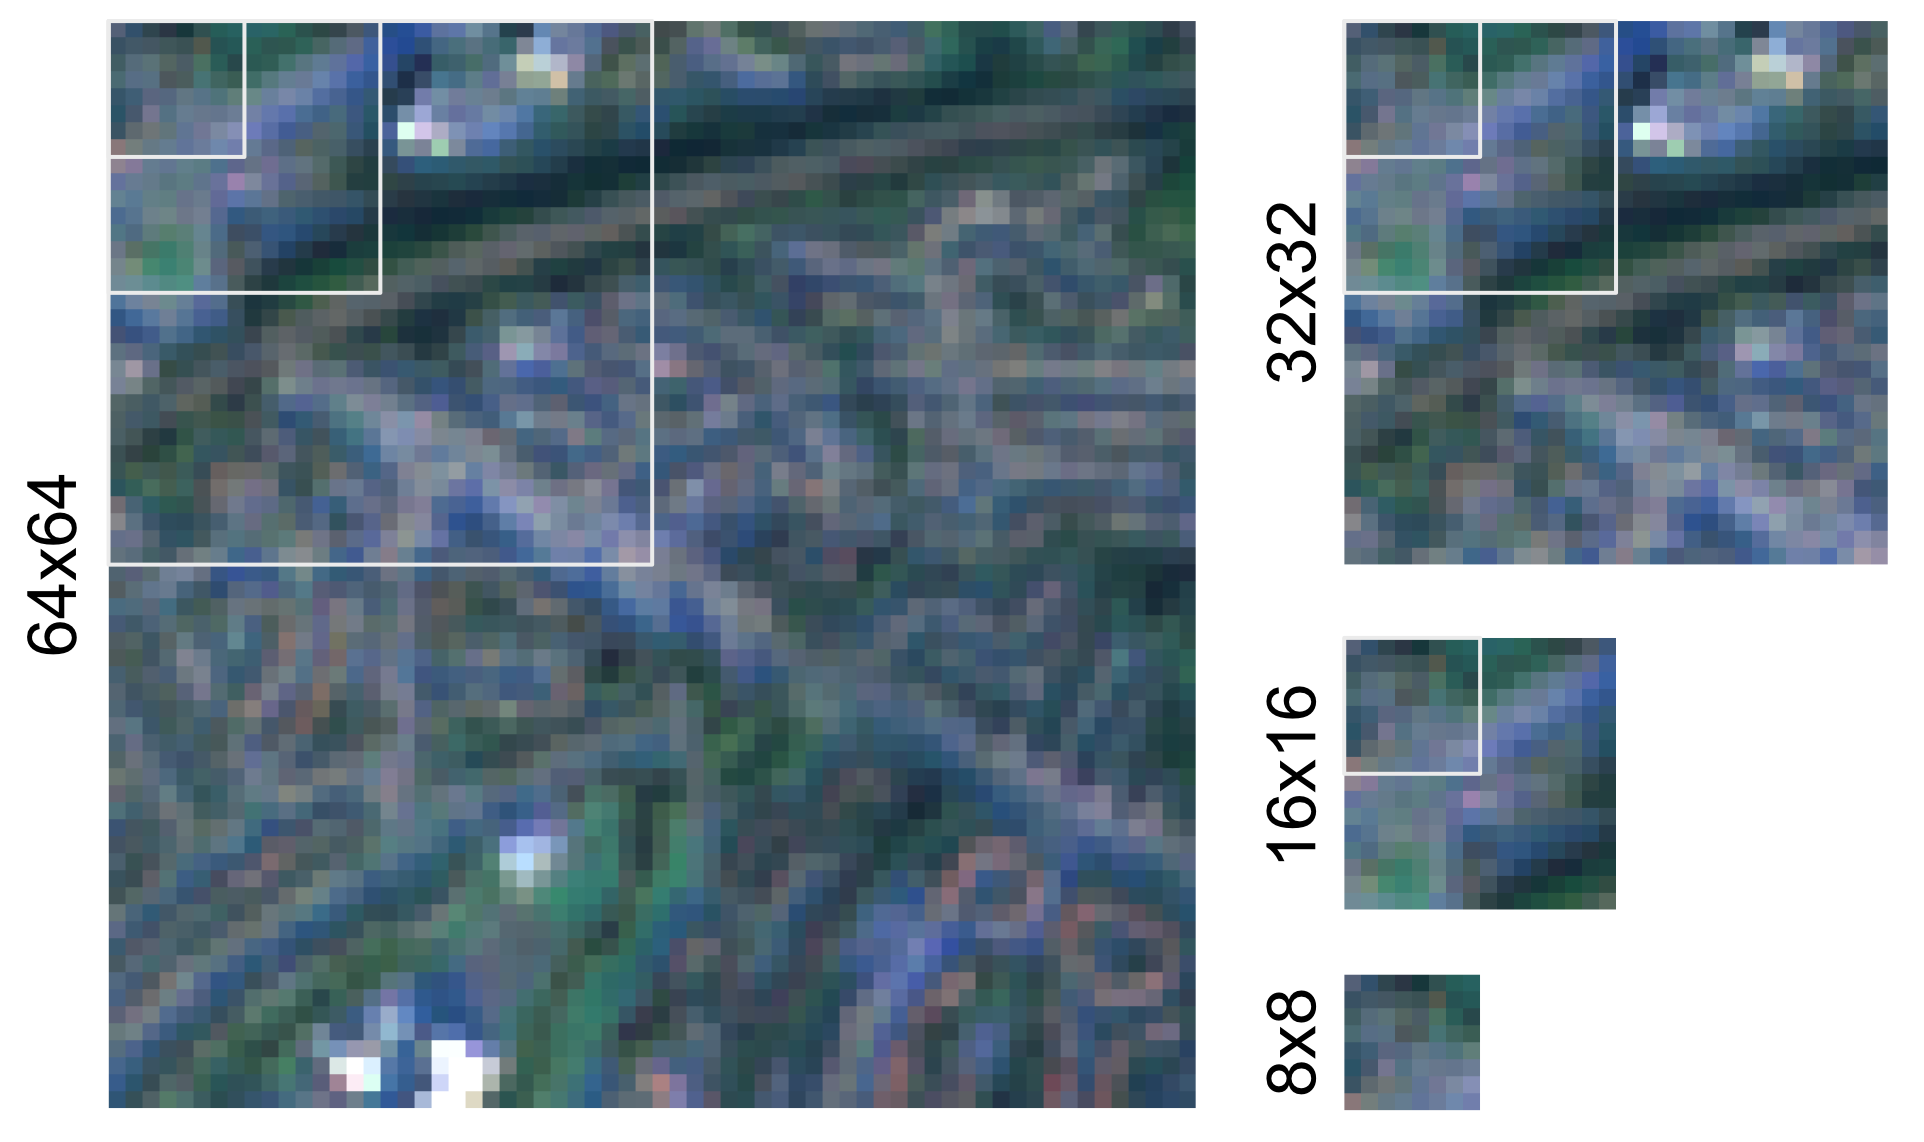
\includegraphics[width=.8\linewidth]{fig/chips.png}
    \caption{Illustration of the selected chip sizes using the Sentinel 2 cloud-free mosaic. Each of the chips also shows the sizes of the smaller options as a white outline.}
    \label{fig:chips}
\end{figure}



\subsubsection{Data (spatial) augmentation}

% Sliding

% 250 words

As mentioned above, certain chip sizes, in combination with the signature geometry and a
requirement to keep them exclusively within a single class, may result in an
insufficient amount of training data for some signature types. Under-sampling like this
one can be a serious problem, that is not unique to spatial modelling. However, the
traditional augmentation methods are not entirely applicable here. For example, in an
image classification problem trying to determine if there is a cat or a dog on an image,
we can flip the picture along y axis, add some rotation or zoom to get more versions of
the same image and expand the set of training data. Neither of these methods is
applicable to the spatial problems. Flipping or rotating the image would break the
natural light conditions, while zooming in would change the scale of urban environment
we are attempting to capture. On the other hand, the geographical nature of the problem
allows us to use spatial augmentation technique we call \textit{sliding}.

Sliding can be seen as overlapping sampling. Instead of overlaying a grid of chips over
target geometry and using each pixel only once, we take the initial grid and slide it a
few pixels horizontally and vertically as illustrated on a figure \ref{fig:sliding}. If
the boundary of a slid chip is fully within a signature geometry, it is added to the
pool of chips to be used. This process is done repeatedly to ensure that each class has
a reasonable amount of chips to work with.

It is to be noted, that sliding can cause a data leakage (sequences of pixel being
present in both training and validation sets) if done before splitting the data into
training and validation subsets. Therefore, we first create the initial grid, subdivide
it spatially into four parts (40\% for CNN training, 10\% for CNN validation, 40\% for
probability modelling training, 10\% for probability modelling validation) and apply
sliding within each part to avoid any pixels being shared among chips from different
sets.

\begin{figure}
    \centering
    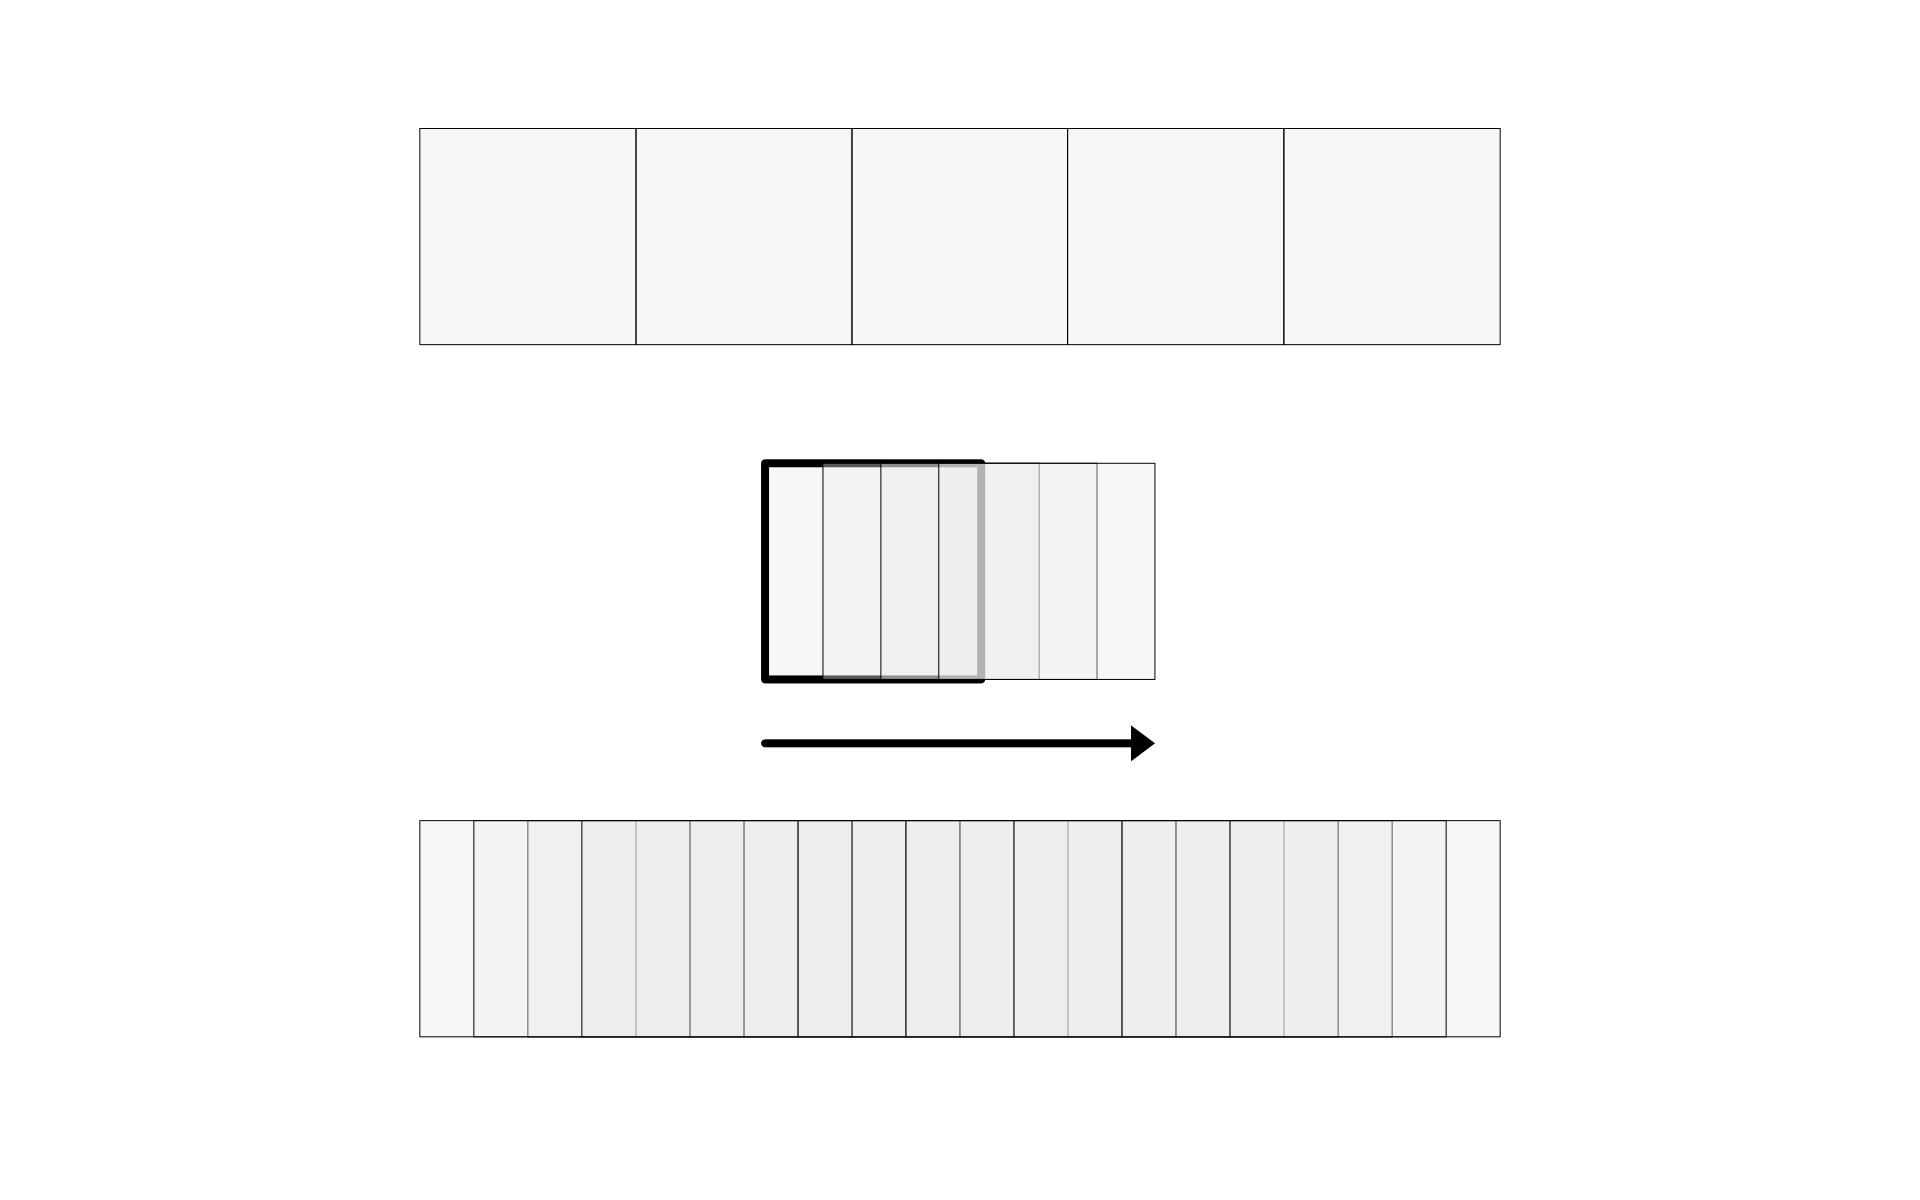
\includegraphics[width=.8\linewidth]{fig/sliding.png}
    \caption{Diagram illustrating the sliding mechanism in one direction. The first row shows the initial non-overlapping grid, the last one final overlapping set of chips. The same approach is then also applied vertically.}
    \label{fig:sliding}
\end{figure}


\subsubsection{Model architecture}

% 500 words

% Overall content of the section

Architecture of each model is composed of two parts. First is the CNN predicting a
probability that a chip belongs to a class (or a proportion of a chip covered by a
class). Second is the machine learning modelling, taking the output of the CNN and
predicting the dominant class. This section describes each of these in detail. It is to
be noted, that contrary to the majority of deep learning-focused research articles, the
actual architecture of CNN is not of a particular interest in this paper. It is assumed
that the effect of geographic decisions will show similar behavior no matter the
architecture (within some limits). This work therefore uses EfficientNetB4 pre-trained
on ImageNet dataset. An appendix \ref*{sec:appendixA} shows a brief comparison of
several standard neural network architectures and their performance on a subset of data
to illustrate the point. The top layer of the pre-trained model is then replaced by a
custom sequence of dense layers described below.

% Standard image classification

The default approach is a standard image classification problem, using the sets of chips
that are fully within a single signature types, both with and without augmentation using
sliding. The custom top layer of the pre-trained CNN then contains a Global Average
Pooling (2D) layer, a dense layer with ReLu activation and 256 neurons, and a dense
layer with the softmax activation and number of neurons equal to a number of classes
(12). A result for a single chip is a an array of a length 12 containing probabilities
that a chip belongs to each class. The sum of all probabilities is 1.

% Multi-output regression

However, there is one more option how to tackle the problem, apart from the image
classification. When we relax the requirement that every chip must be fully within
boundaries of a single signature type, we end up with chips encoding proportions of area
belonging to each class. Instead of a single label per chip, we now deal with an array.
This can be beneficial from the geographical perspective as such chips now inherently
encode co-location of individual signature types and a model can use this information
during the prediction. As signature types usually tend to neighbor only a subset of
other classes (e.g., Urbanity never neighbors Wild Countryside), we can assume that an
information on co-location can positively impact the resulting performance. For these
reasons, we include a set of chips sampled from a grid crossing the boundaries of
signature types (using the same chip sizes as before) and adapt the CNN for the
multi-output regression problem instead of image classification one. That means that the
top layer is composed of a Global Average Pooling (2D) layer a dense layer with ReLu
activation and 256 neurons and a dense layer with the sigmoid activation and a number of
neurons equal to a number of classes (12). The result for a single chip is a similar
array but containing predicted proportions. The sum of all proportions can be anything
within 0 and 12x1.

% Spatial modelling of probabilities TODO: Dani, from this section below are your bits.

\subsubsection{Performance metrics}

% 500 words

% Traditional non-spatial

% Explicitly spatial metrics % Why % Which ones % Why those? (ideally link to Miguel's
%paper suggestions)

\subsubsection{Summarizing experiments}

% 250 words

% explanation of regression approach